\documentclass{beamer}

\usepackage[ngerman]{babel}
\usepackage{array}
\usepackage{listings}
\usepackage{caption}
\usepackage{dirtytalk}
\usepackage{graphicx}

\beamertemplatenavigationsymbolsempty

\definecolor{codegreen}{rgb}{0,0.6,0}
\definecolor{codegray}{rgb}{0.5,0.5,0.5}
\definecolor{codepurple}{HTML}{C42043}
\definecolor{backcolour}{HTML}{F2F2F2}
\definecolor{bookColor}{cmyk}{0,0,0,0.90}  
\color{bookColor}

\lstset{upquote=true}

\lstdefinestyle{mystyle}{
    backgroundcolor=\color{backcolour},   
    commentstyle=\color{codegreen},
    keywordstyle=\color{codepurple},
    numberstyle=\footnotesize\color{codegray},
    stringstyle=\color{codepurple},
    basicstyle=\footnotesize,
    breakatwhitespace=false,         
    breaklines=true,                 
    captionpos=b,                    
    keepspaces=true,                 
    numbers=left,                    
    numbersep=-10pt,
    showspaces=false,                
    showstringspaces=false,
    showtabs=false,      
}
\lstset{style=mystyle} 

\title{Population Genetics}
\subtitle{Peerteaching KW24}
\author{Samuel Hehn \\ Swastik Kashyap}
\institute{Universität Tübingen}
\usetheme{Goettingen}
\date{\today}

\begin{document}

    {
    \setbeamertemplate{sidebar right}{}
    \begin{frame}
        \titlepage
    \end{frame}
    }

    {
    \setbeamertemplate{sidebar right}{}
    \begin{frame}
        \frametitle{Inhalt}
        \tableofcontents
    \end{frame}
    }

    \section{Introduction}
        \begin{frame}
            \frametitle{Introduction}
            Population genetics aims to infer details of evolutionary processes based on the current population's genetic composition. \\
            Subfield of Genetics 
        \end{frame}

    \begin{frame}
        \frametitle{Single Nucleotide Variant(SNV)}
        A single-nucleotide variant (SNV) is a variation in a single nucleotide that occurs at a specific position in the genome. This may be rare or common in a population. \\
    \end{frame}

    \begin{frame}
        \frametitle{Single Nucleotide Polymorphism(SNP)}
        A single-nucleotide polymorphism (SNP) is a SNV that occurs in a significant proportion (typically $>$ 1\%) of a population. \\
        Polymorphisms describe sites (nucleotide positions, etc.) that are variable within a species; divergence describes sites variable between species.
    \end{frame}
    
    \section{Basic models of population growth}
    \begin{frame}
        \frametitle{Basic models of population growth}
        $r = \frac{s(T)-s(T_0)}{s(T_0)}$ \\
        where s(T) is the population size at time T and s(T0) the size of the initial population at time T0. 
    \end{frame}

    \section{Alleles and Ploidy}
    \begin{frame}
        \frametitle{Alleles and ploidity}
        An allele is the variant form of a given gene found at the same chromosomal location.
        \\
        Ploidy is the number of sets of chromosomes in a cell and hence the number of possible alleles for genes.
    \end{frame}

    \begin{frame}
        \frametitle{Haploid and Diploid}
        Haploid Cells:
        Haploid cells have half the number of chromosomes (n) as diploid - germ cells Result of meiosis\\
        Example: sperm and egg cells\\
        Diploid Cells:
        Diploid cells contain two copies of each chromosome (2n) - somatic cells Result of mitosis\\
        Example: skin cells
    \end{frame}

    \begin{frame}
        \frametitle{Haploid Reproduction Model}
       - Assume constant population size\\
       - Each gene i in generation t + 1 is found by randomly choosing a predecessor gene g in generation t. This implies, that it is possible that one gene can have more than one offspring.\\
       - Any gene in generation t not chosen “dies out”.
        \begin{figure}
         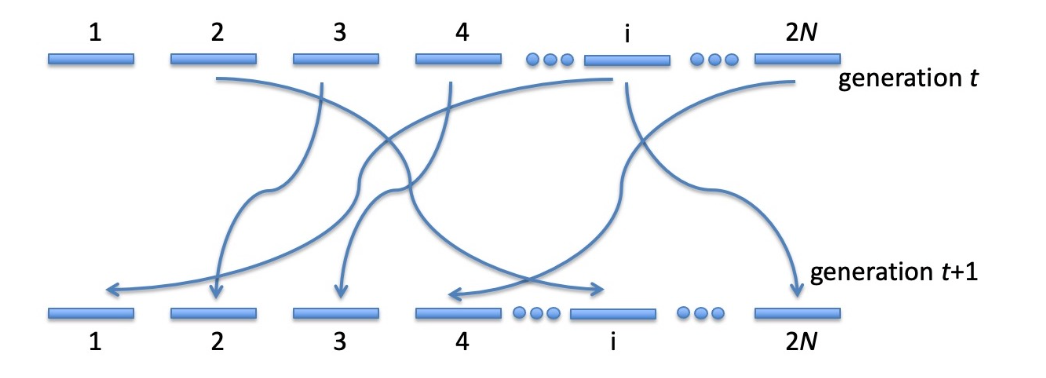
\includegraphics[width=\textwidth]{haploidRep.png}
            \caption{Haploid reproduction model}
        \end{figure}
    \end{frame}

    \begin{frame}
        \frametitle{Diploid populations}
        Assumptions - 
        Species has 2 Sexes, Male ans Female. \\
        Each individual has 2 copies of each gene, a gene is chosen for each parent with equal odds \\
        In this model, each gene has one parent gene and each individual has two parents.\\
        For large values of N, Nf and Nm, one can approximate the diploid model by the haploid model.
        Thus, we will only consider the haploid model.\\
        \begin{figure}
            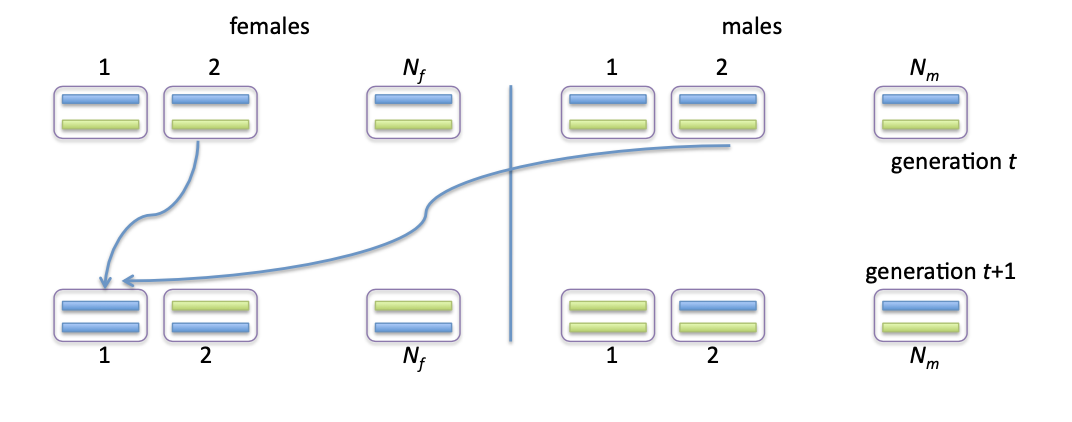
\includegraphics[width=0.8\textwidth]{diploidRep.png}
               \caption{Diploid reproduction model}
           \end{figure}
    \end{frame}

    \begin{frame}
        \frametitle{Haplotypes and Genotypes}
        Haplotype: A haplotype is a sequence of an individual’s genome that occurs together on one or two homologous copies of a chromosome.\\
        Genotype: The two alleles at the same site on two homologous chromosomes form the genotype at that site. We denote that by ‘P$|$Q’, if ‘P’ and ‘Q’ are the alleles, respectively.
        Example \\
        An individual has the two haplotypes \\
        A T T G A C A T C \\
        A C T G A C A C T \\
        Then the genotype at the first site is A$|$A, at the second site T$|$C, and so on. \\
        Task- Show the full genotype of the individual.
    \end{frame}

    \begin{frame}
        \frametitle{Homozygous and Heterozygous}
        A site c is called homozygous if the genotype consists of two identical alleles at c. The site c is called heterozygous if the genotype consists of two different alleles at c. \\
        Task- for an individual that has the two haplotypes \\
        A T T G A C A T C \\
        A C T G A C A C T \\
        give the set of homozygous and heterozygous sites. 
    \end{frame}

    \section{Calculating Populations}
        \begin{frame}
            \frametitle{Calculating decendants}
            What is the probability of any gene $i$ to have at least one decendant (It does not \say{die out})? \\
            \onslide<2->{
                We look at the inverse probability, a gene has no decendants.
            }
            \onslide<3->{
                \[
                    \implies \mathbb{P}_{\text{Poisson}}(X = k) = \frac{\lambda^{k}}{k!} e^{-\lambda}
                \]
            }
            \onslide<4->{
                Since the population keeps it size from generation to generation, the average number of decendants per gene is 1.
            }
            \onslide<5->{
                \[
                    \implies \mathbb{P}_{\text{Poisson}}(X=k) = \frac{1}{k!}e^{-1}
                \]
            }
            \onslide<6->{
                No decendants: ($k=0$)
                \[
                    \mathbb{P}_{\text{Poisson}}(X=0) = e^{-1} \approx 0.37
                \]
            }
            \onslide<6->{
                At least one decendant: 
                \[
                    1 - 0.37 \approx 0.63
                \]
            }
        \end{frame}

        \begin{frame}
            \frametitle{Calculating decendants}
            \framesubtitle{Why is this useful?}
            What was the size of a population of $10\,000$ genes $t=15$ generations ago? \\
            \onslide<2->{
                \[
                    10\,000 \cdot 0.63^{15} 
                    \onslide<3->{\approx 10}
                \]
            }
            \onslide<4->{
                So a population of $10\,000$ genes would have most likely evolved from just $10$ genes over a course of 15 generations. \\
            }
            \vspace*{1cm}
            \onslide<5->{
                This means we can now find out how many generations back there was just one individual (the most recent common ancestor of our whole population).
            }
        
        \end{frame}

    \section{The coalescent process}

        \begin{frame}
            \frametitle{The coalescent process}
            \say{\textit{to coalesce}}: grow together, to join, to fuse


            \begin{definition}[coalescent event]<2->
                \textit{
                    If traversing the sequence-transmission paths backward in time,
                    two sequence transmission paths intersect at some sequence,
                    the paths coalesce at that intersection point. \\
                    This is called a coalescent event.
                }
            \end{definition}
        
            \begin{block}{Basic idea}<3->
                \begin{itemize}
                    \item<4-> Start with present-day generation
                    \item<5-> Construct previous generations
                    \item<6-> By randomly choosing parents in the previous generation
                \end{itemize}
            \end{block}
        \end{frame}

        \begin{frame}
            \frametitle{The coalescent process}
            \framesubtitle{Example}
            \only<2>{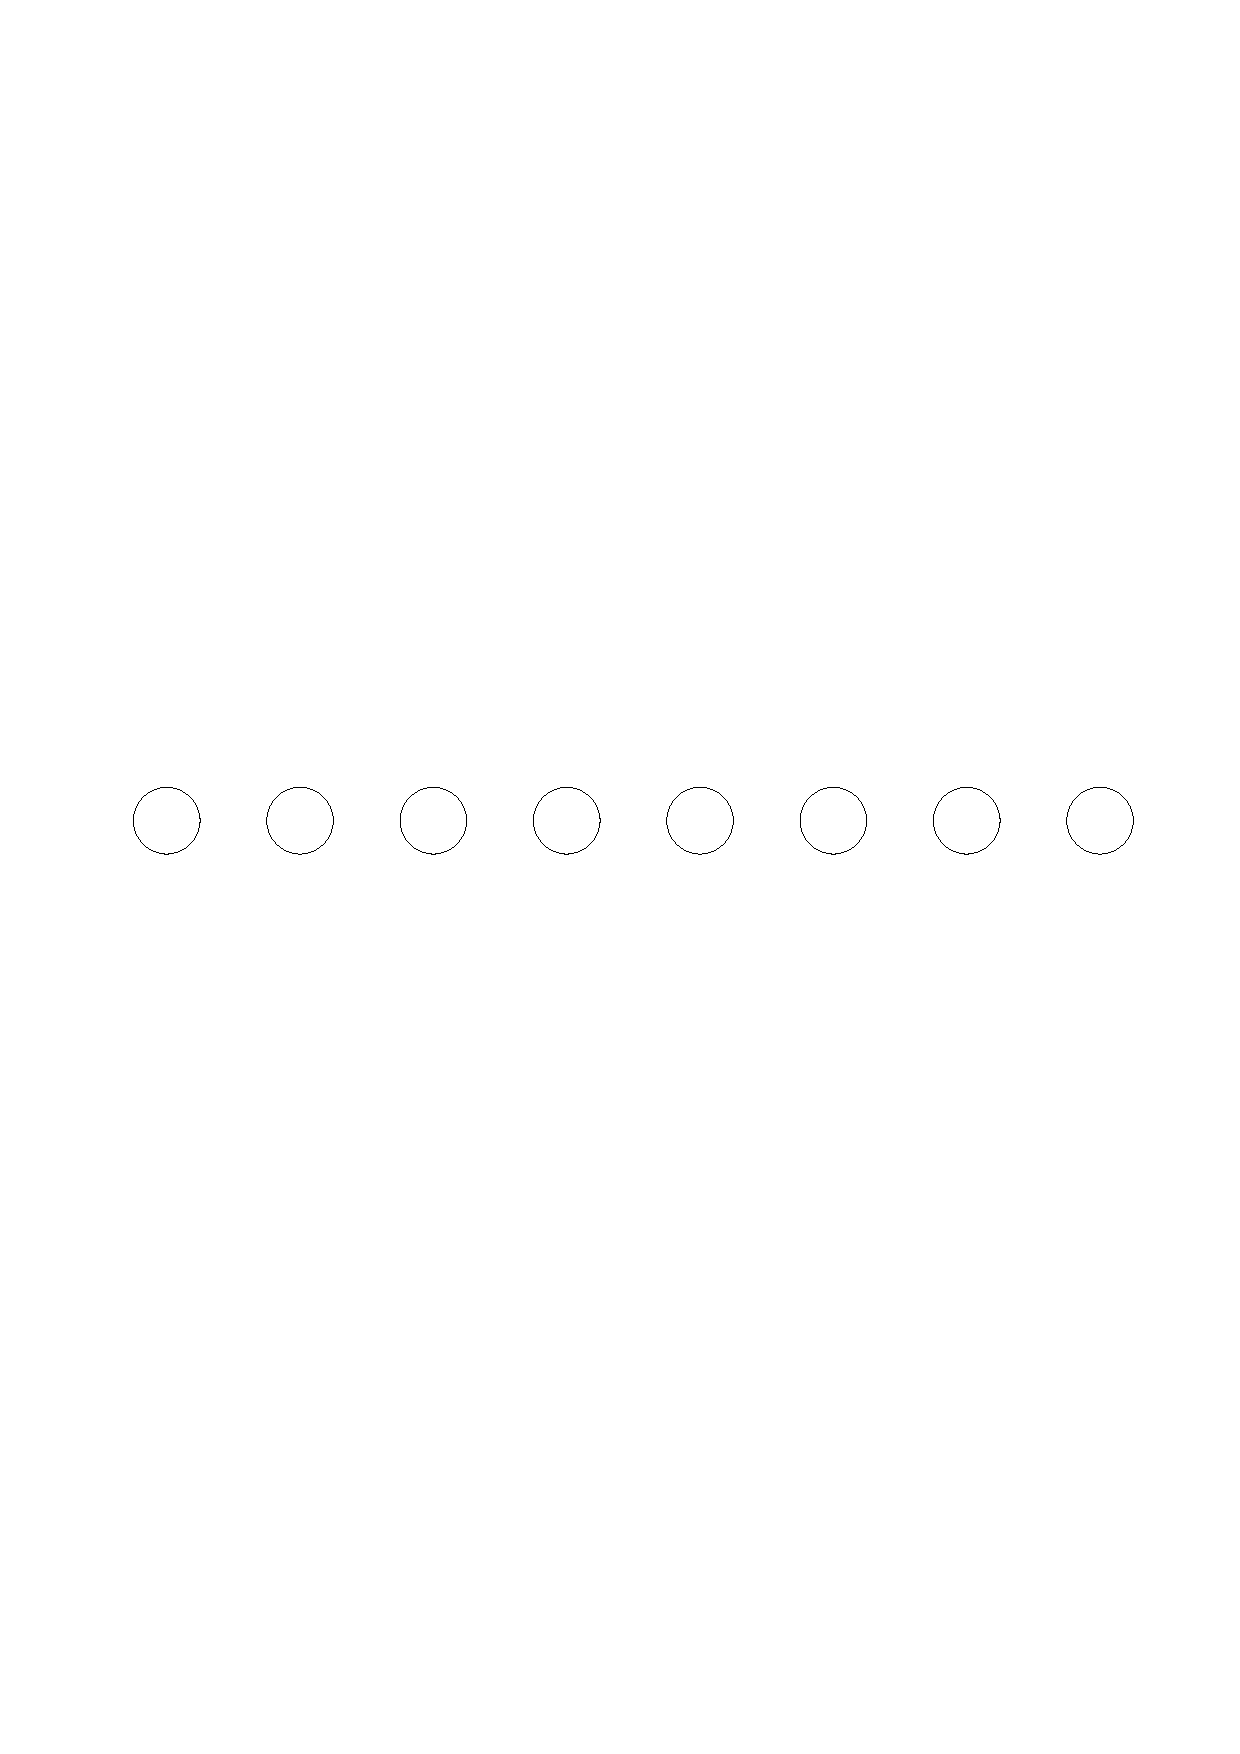
\includegraphics[page=1, width=\textwidth]{figures/coalescent_process.pdf}}
            \only<3>{\includegraphics[page=2, width=\textwidth]{figures/coalescent_process.pdf}}
            \only<4>{\includegraphics[page=3, width=\textwidth]{figures/coalescent_process.pdf}}
            \only<5>{\includegraphics[page=4, width=\textwidth]{figures/coalescent_process.pdf}}
            \only<6>{\includegraphics[page=5, width=\textwidth]{figures/coalescent_process.pdf}}
            \only<7>{\includegraphics[page=6, width=\textwidth]{figures/coalescent_process.pdf}}
            \only<8>{\includegraphics[page=7, width=\textwidth]{figures/coalescent_process.pdf}}
            
        
        \end{frame}

    \section{The standard coalescent model}
        \begin{frame}
            \frametitle{Coalescence of 2 genes}
            Considering a haploid model with $n$ genes. \\
            For two present day genes $i$ and $j$, when did they coalesce? \\
            \onslide<2->{We want two know two things:}
            \begin{enumerate}
                \item<3-> When did the two genes coalesce? \\
                      \onslide<4->{$\rightarrow$ Who is their common ancestor}
                \item<5-> How long is the waiting time until the two genes coalesced? \\
                      \onslide<6->{$\rightarrow$ How many generations back is their common ancestor?}
            \end{enumerate}
        \end{frame}

        \begin{frame}
            \frametitle{Coalescence of 2 genes}
            \framesubtitle{When did the two genes coalesce? }
                \onslide<2->{
                    We select a random ancestor for each individual: \\
                }
                \onslide<3->{
                    Probability to select the right ancestor of $i$ is $1$, since there are no requirements. \\
                }
                \onslide<4->{
                    Probability to select the right ancestor of $j$ is
                }
                \onslide<5->{
                    $$P(T_{2} = 1) = \frac{1}{n}$$
                    since we need to "hit" the ancestor we've chosen for $i$.
                }
        \end{frame}

        \begin{frame}
            \frametitle{Coalescence of 2 genes}
            \framesubtitle{How long is the waiting time until the two genes coalesced?}
            \onslide<2->{
                What is the Probability that the common ancestor is in Generation $t$? \\
            }
            \onslide<3->{
                ($t-1$ failures following one success)
                \[
                    P(T_{2} = t) = 
                    \onslide<4->{\left( 1 - \frac{1}{n} \right)^{n-1}}
                    \onslide<5->{\cdot \left( \frac{1}{n} \right)}
                \]
            }
        \end{frame}

        \begin{frame}
            \frametitle{Coalescence of 2 genes}
            \framesubtitle{Exercise}
            Let's assume $n = 50$ \\
            What is the probability that two genes coalesce exactly 5 generations in the past? \\ 
                \[
                    P(T_{2} = 5) =
                    \onslide<2->{\left(1 - \frac{1}{50}\right)^{5-1} \cdot \frac{1}{50}}
                    \onslide<3->{\approx 0.01845 = 1.845\%}
                \]
        \end{frame}

        \begin{frame}
            \frametitle{Coalescence of 2 genes}
            \framesubtitle{Exercise}
            Let's assume $n = 50$ \\
            What is the probability that it takes them at least 5 generations to coalesce? \\ 
                \[
                    P(T_{2} > 5) =
                    \onslide<2->{\left(1 - \frac{1}{50}\right)^{5}}
                    \onslide<3->{\approx 0.903921
                    = 90.392\%}
                \]
        \end{frame}

    \section{Most recent common ancestor}
    \begin{frame}
        \frametitle{Most recent common ancestor(MRCA)}
        How many generations back is the most recent common ancestor (MRCA) of two present-day genes?
    \end{frame}

    \begin{frame}
        \frametitle{Wright Fisher Model}
        Key assumptions of the Wright-Fisher model: \\
        1. Discrete and non overlapping generations. \\
        2. Constant population size. \\
        3. Haploid individuals \\
        4. All individuals are equally fit. \\
        5. The population has no geographic or social structure\\
        6. No recombinations of genes (or sequences)



    
        
    
    \end{frame}


\end{document}
